\documentclass[ngerman,ph]{beamer}

\usepackage{babel}
\usepackage[utf8]{inputenc}
\usepackage[T1]{fontenc}
\usepackage{lmodern}
\usepackage{geometry}
\usepackage{graphicx}
\usepackage{amsmath}
\usepackage{multimedia}

\newcommand{\diff}{\mathrm{d}}


\title{Thermodynamik schwarzer Löcher}
\institute{Fakultät für Physik}
%\subtitle{Im CD der Universität Regensburg}
\author{Tamara Szecsey}

\begin{document}
	
	\begin{frame}
		\maketitle
		\begin{figure} [h] 
			\begin{center}
				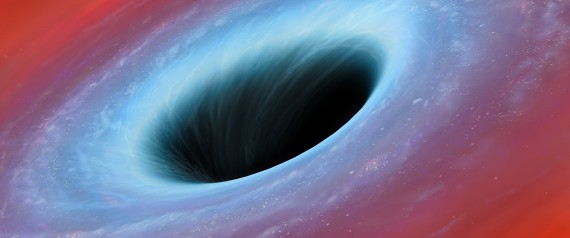
\includegraphics[width=0.7\textwidth]{n-117451542-large570}
			\end{center}
		\end{figure}
	\end{frame}
	
	\begin{frame}
		\tableofcontents
	\end{frame}
	
	\section{Was ist Informationsentropie?}
	\begin{frame}{Informationsentropie}
		\begin{block}{}
			Die Entropie zählt wieviele Mikrozustände eines Systems einen Makrozustand bilden. 
			
			Beispiel: Wurf von zwei W6 Würfeln.
		\end{block}
		
		\begin{block}{}
		Wie viele Ja-Nein-Fragen muss man beantworten, um das Ergebnis zu bekommen?
		(Im Falle von genau zwei möglichen Ausgängen.)
		Beispiel: Münzwurf hat die Informationsentropie von 1 Bit.	
		\end{block}
%		\hfill
		\begin{figure} [h] 
			\begin{center}
				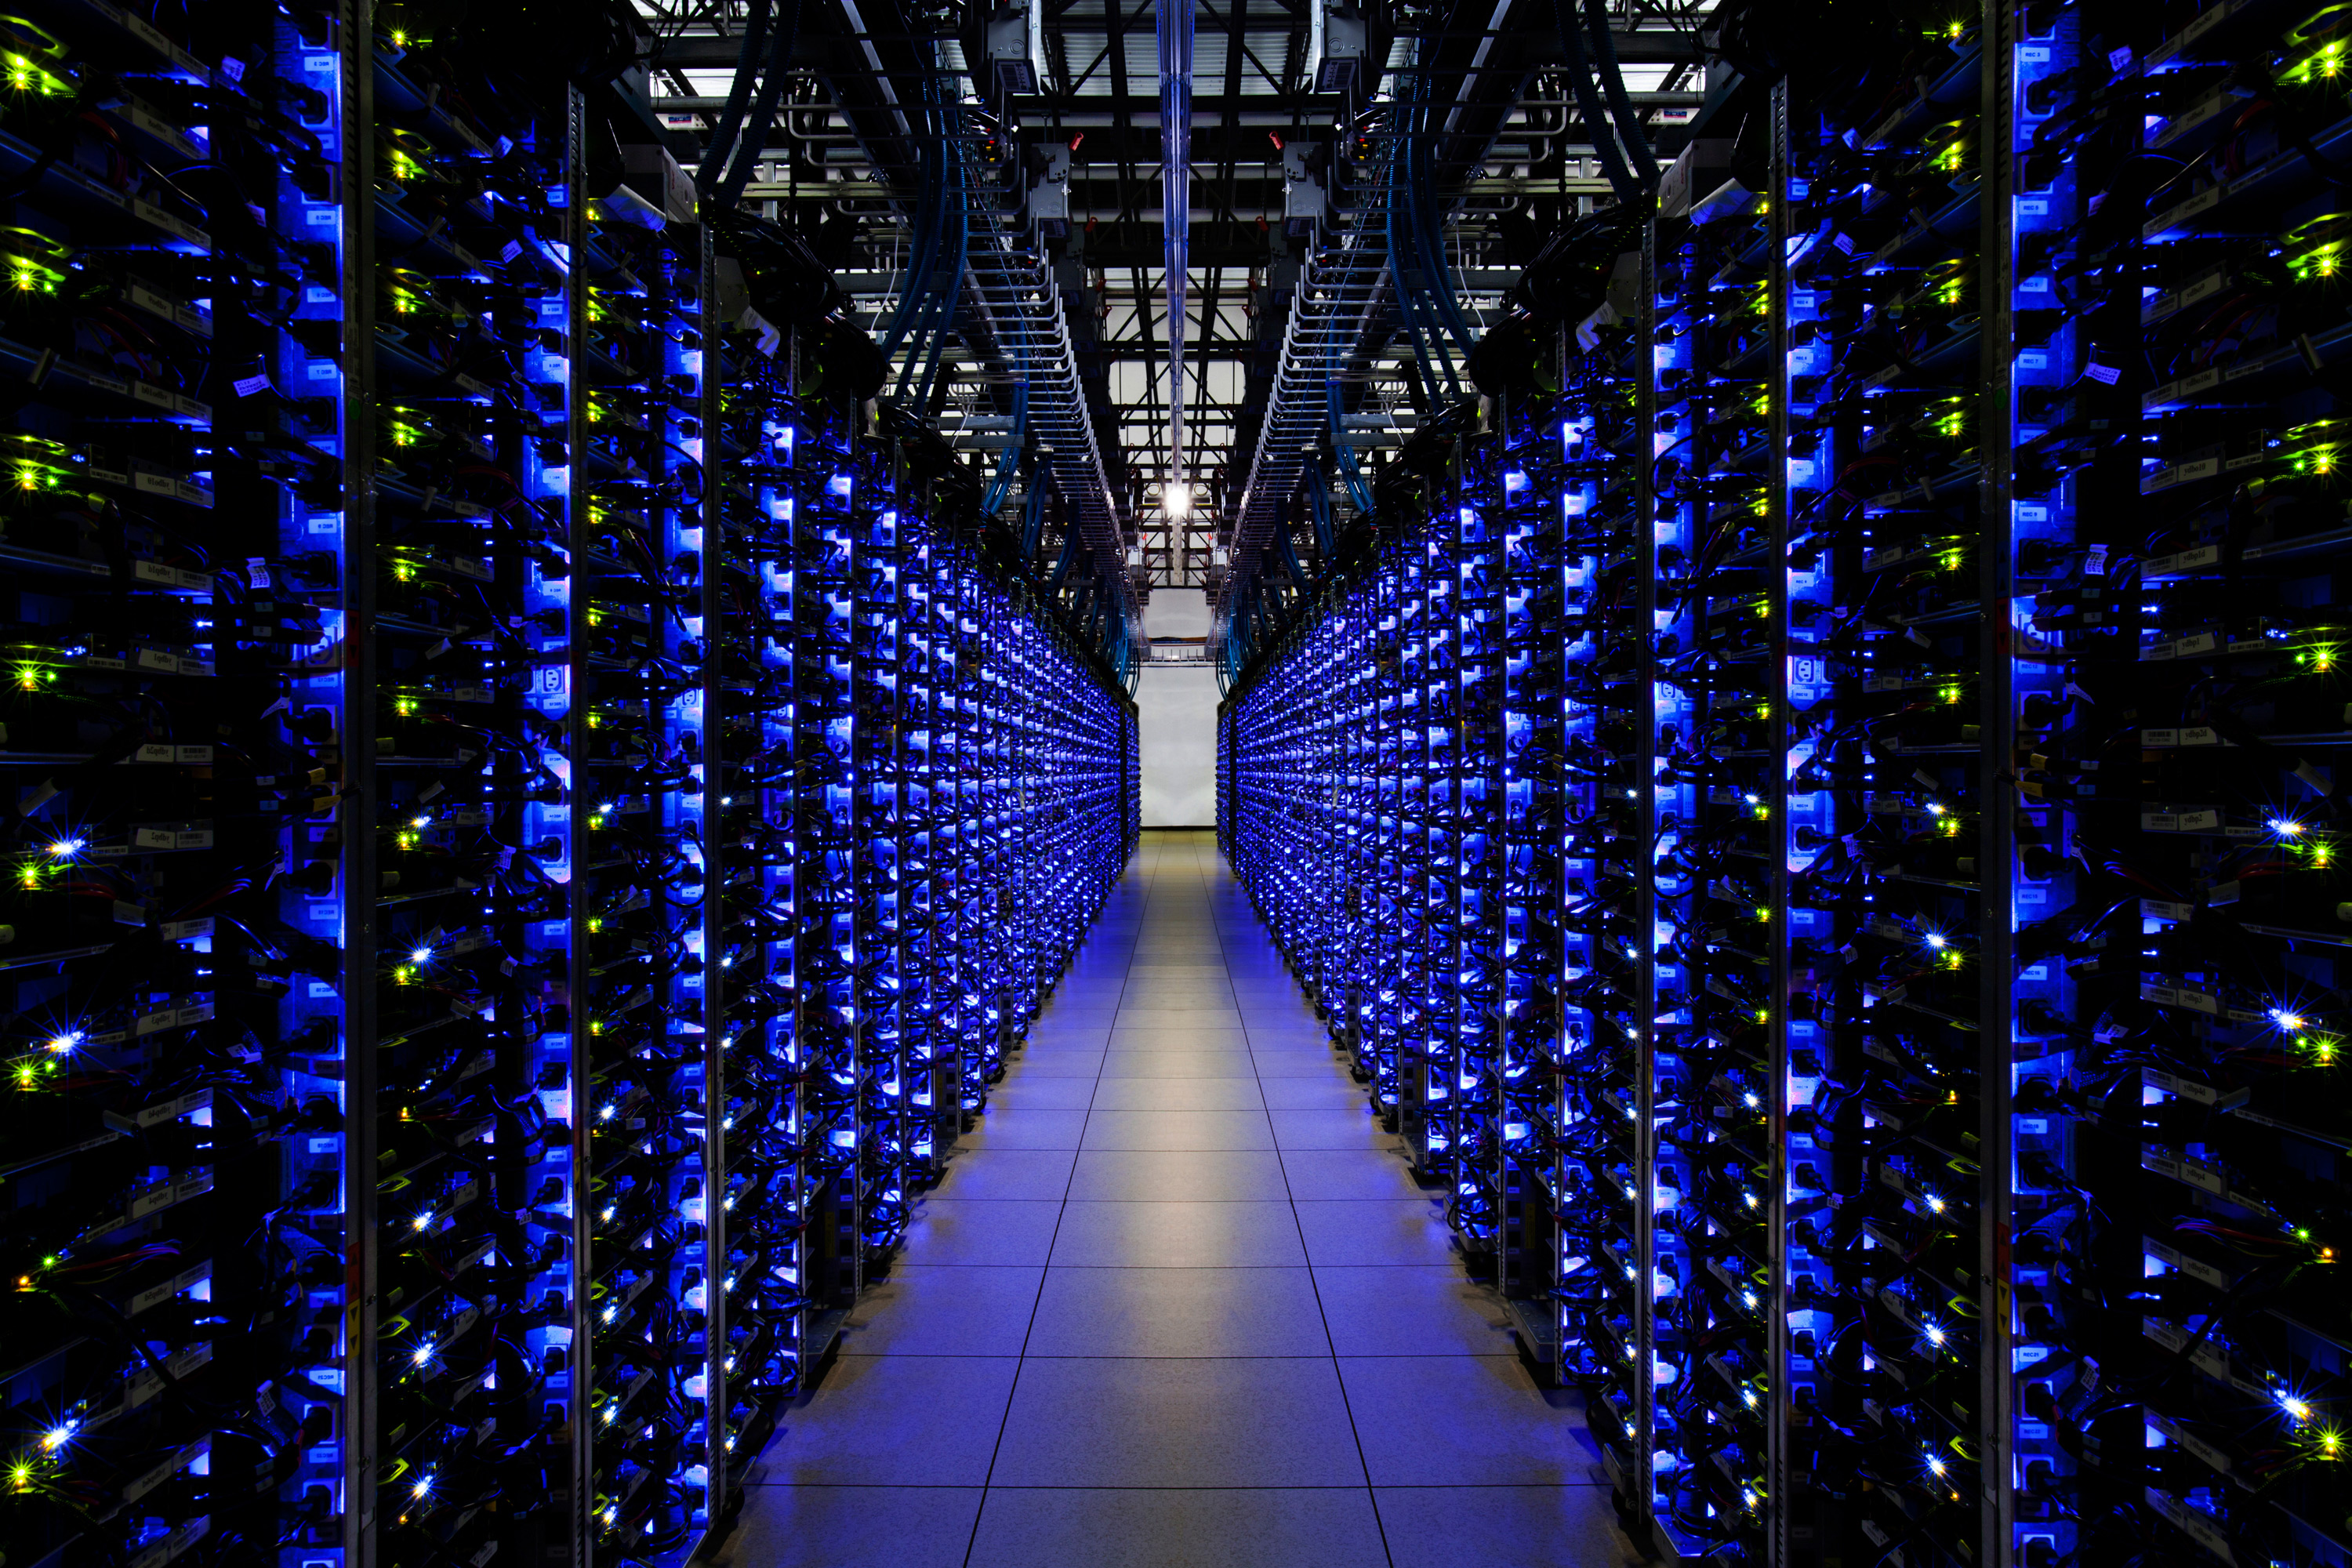
\includegraphics[width=0.5\textwidth]{Server}
			\end{center}
		\end{figure} 	 	%http://www.google.com/about/datacenters/gallery/images/_3000/IDI_018.jpg	
		\hfill
	\end{frame}
	
	\section{Die drei Hauptsätze}
	\begin{frame}{Der Nullte Hauptsatz der Thermodynamik}
		\begin{center}
			\Large{Die Hawkingstrahlung} 
		\end{center}
		\begin{figure} [h] 
			\begin{center}
				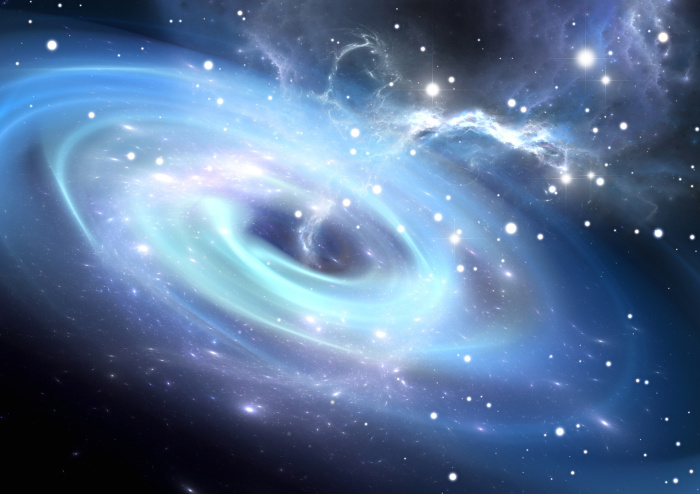
\includegraphics[width=0.5\textwidth]{Hawkingstrahlung}
			\end{center}
		\end{figure} %http://www.spektrum.de/fm/912/thumbnails/SchwarzesLoch_fotolia64583984_PeterJurik.1584161.jpg.1584174.jpg		
	\end{frame}
	\begin{frame}{Der Nullte Hauptsatz der Thermodynamik}	
		\begin{figure} [h] 
			\begin{center}
				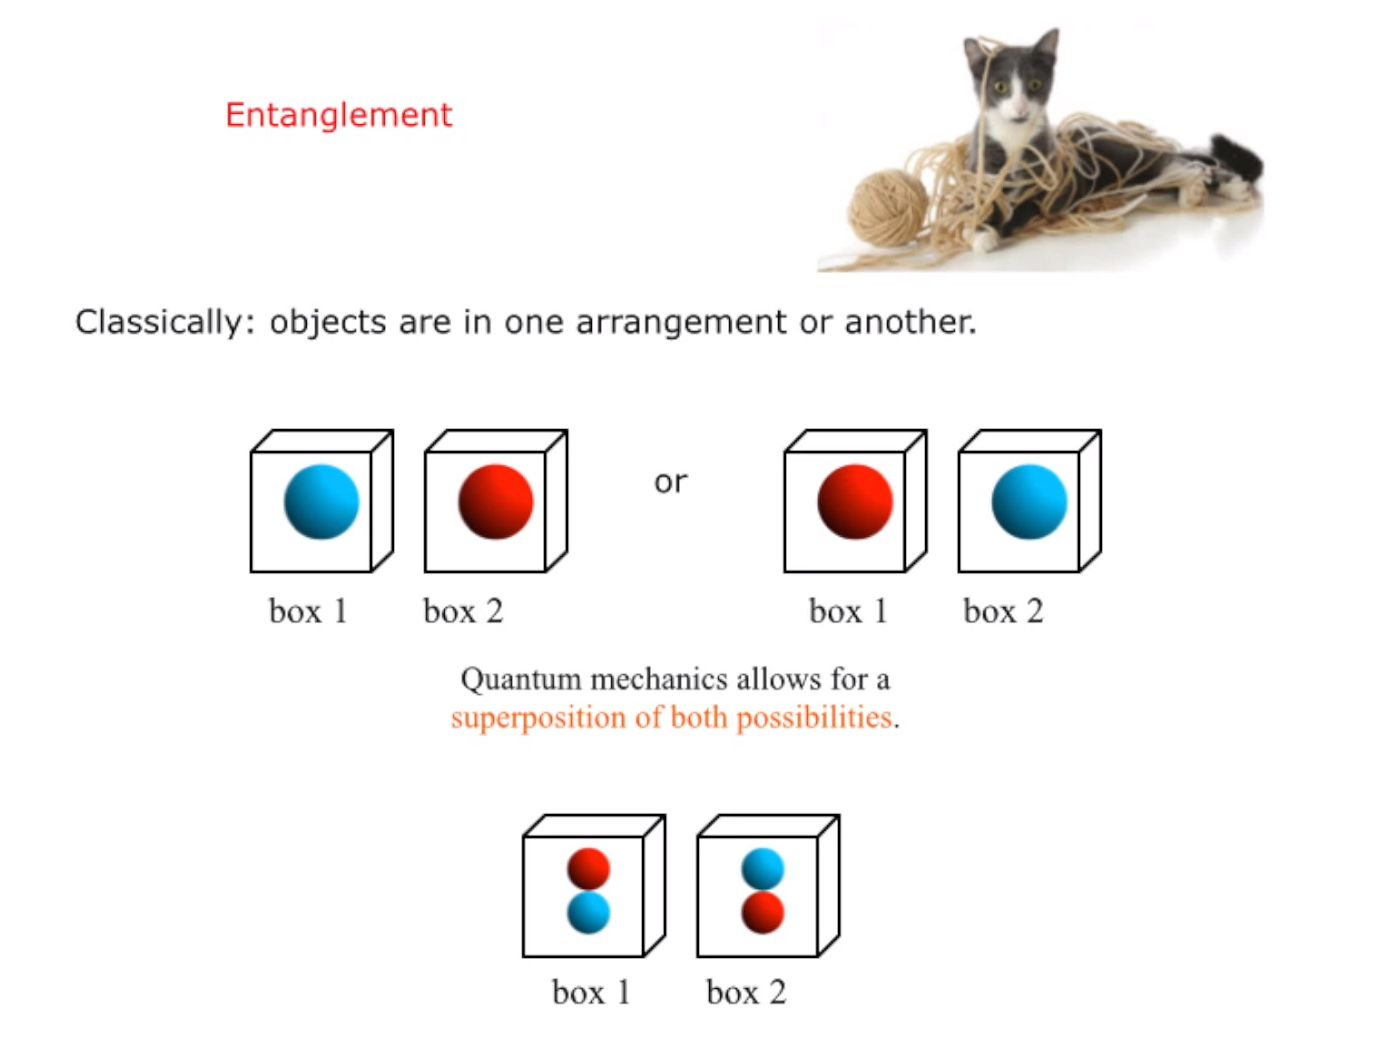
\includegraphics[width=0.8\textwidth]{entanglement}
			\end{center}
		\end{figure} 	%https://www.youtube.com/watch?v=_8bhtEgB8Mo&feature=youtu.be
	\end{frame}
	\begin{frame}{Der Nullte Hauptsatz der Thermodynamik}
		\begin{center}
			\Large{Die Hawkingstrahlung} 
		\end{center}
		\begin{figure} [h] 
			\begin{center}
				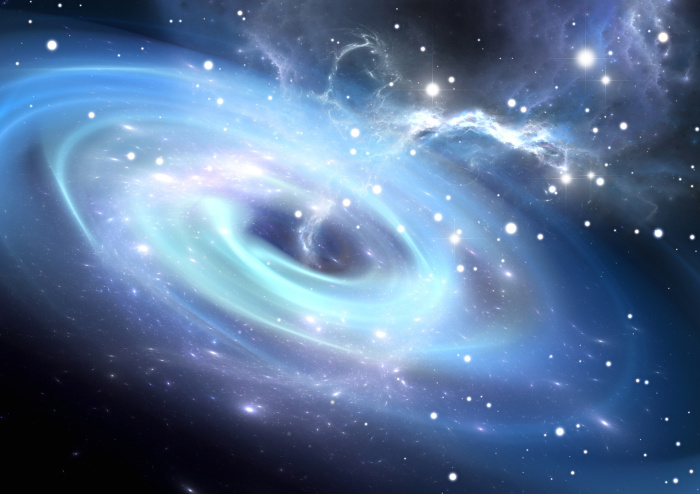
\includegraphics[width=0.5\textwidth]{Hawkingstrahlung}
			\end{center}
		\end{figure} %http://www.spektrum.de/fm/912/thumbnails/SchwarzesLoch_fotolia64583984_PeterJurik.1584161.jpg.1584174.jpg	
		Nullter Hauptsatz besagt nun, dass genauso viel Temperatur aufgenommen werden muss, wie abgestrahlt wird 
		
		$\Rightarrow$ Beschleunigung an der Oberfläche	
	\end{frame}
	
	
	\begin{frame}{Der Erste Hauptsatz der Thermodynamik}
		Der erste Hauptsatz der Thermodynamik besagt Energieerhaltung:
		\begin{align*}
		\Delta U = \Delta Q + \Delta W
		\end{align*}
		\begin{columns}
			\begin{column}{6cm}
				Umgeschrieben:
					\begin{align*}
					\diff E = T\diff S + \diff W
					\end{align*}
				Analogie zu schwarzen Löchern mit Hilfe von Kerr-Neumann Metrik und geschickt gewählten Koordinaten
			\end{column}
			\begin{column}{4cm}
%				\begin{minipage}[l]{0.4\textwidth}
					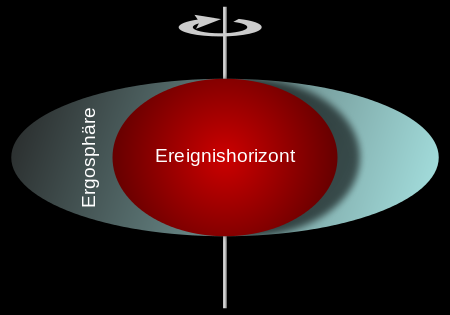
\includegraphics[width=\textwidth]{Kerr-Neumann}
%				\end{minipage} %https://de.wikipedia.org/wiki/Kerr-Metrik (12.01.20016)
				\vfill
			\end{column}
		\end{columns}
	\vfill
	Ergebnis:
		\begin{align*}
		\diff (Mc^2) = \frac{\kappa}{8 \pi G} \diff A + \Omega \diff J - \Phi \diff q
		\end{align*} 	 		
	\end{frame}	

	\begin{frame}{Der Zweite Hauptsatz der Thermodynamik}
		\begin{figure}
			\begin{minipage}[c]{0.45\textwidth}
				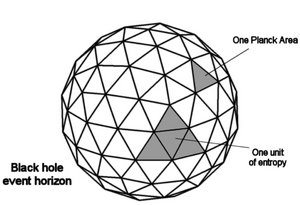
\includegraphics[width=\textwidth]{BHentropy1}
			\end{minipage}
			\hfill
			\begin{minipage}[c]{0.45\textwidth}
				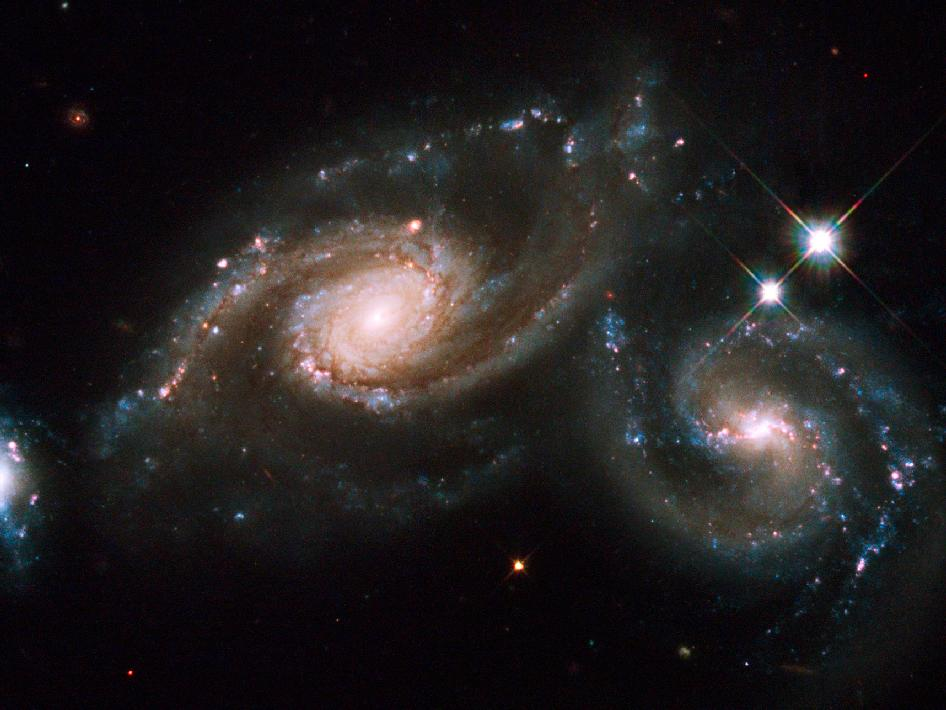
\includegraphics[width=\textwidth]{kollidierendeSHs}
			\end{minipage}
		\end{figure}
%		\begin{figure} [h] 
%			\begin{center}
%				\movie[externalviewer]{vlc}{earthpointofview_wmv}
%			\end{center}
%		\end{figure}
	\end{frame} %quelle: http://www.nasa.gov/mission_pages/hubble/multimedia/arp274_prt.htm
	
	\section{Verdampfung}
	\begin{frame}{Verdampfung/Evaporation}
		\begin{figure} [h] 
			\begin{center}
				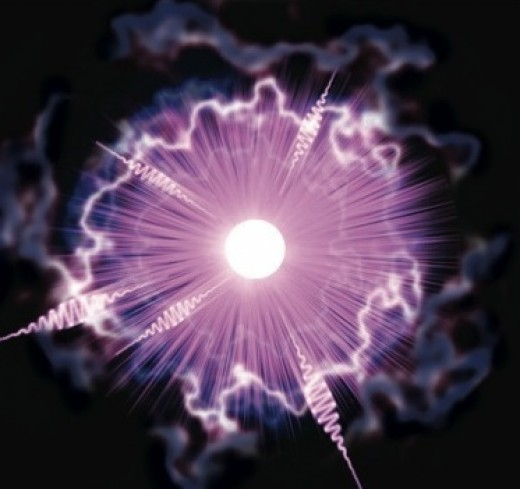
\includegraphics[width=0.5\textwidth]{evaporation}
			\end{center}
		\end{figure}
	 %http://hubpages.com/education/Hawking-Radiation-and-Evaporating-Black-Holes#slide4018139
	\end{frame}
	
	\section{Weitere Betrachtung}
	\begin{frame}{Weitere Betrachtung}
		\begin{figure} [h] 
			\begin{center}
				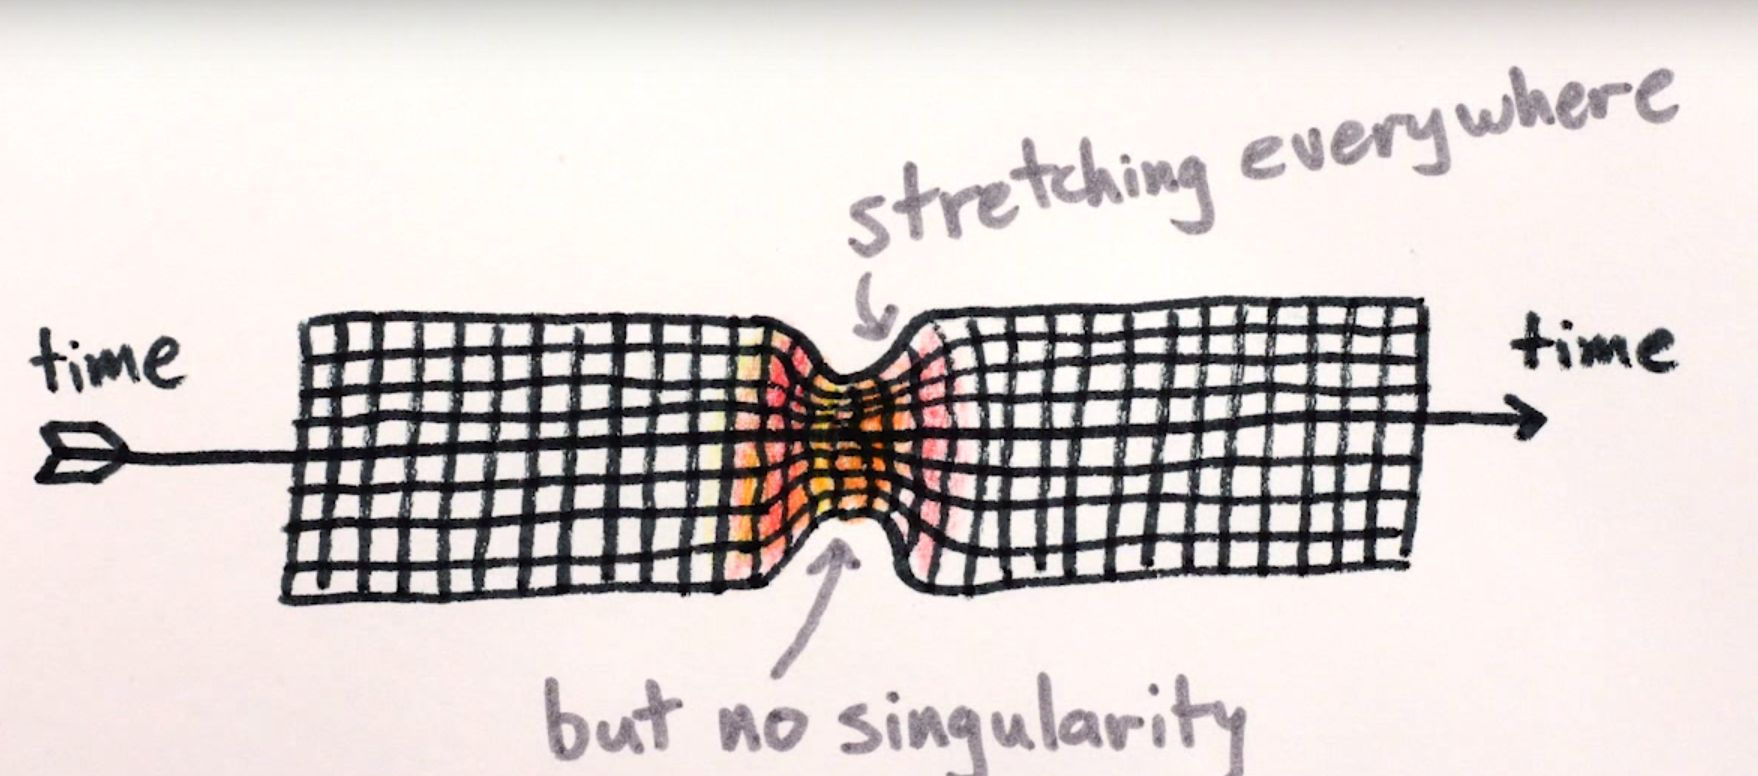
\includegraphics[width=0.5\textwidth]{bounce1}
			\end{center}
		\end{figure} 
%		\begin{figure} [h] 
%			\begin{center}
%				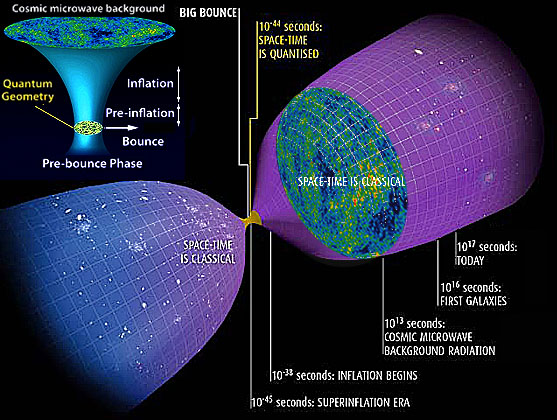
\includegraphics[width=0.5\textwidth]{bounce}
%			\end{center}
%		\end{figure} 
	\end{frame}	
	% http://pics-about-space.com/black-matter-black-holes?p=2#
	\begin{frame}
		\begin{minipage}[c]{\textwidth}
			\huge{Vielen Dank für Eure Aufmerksamkeit!}
		\end{minipage}		
	\end{frame}
\end{document}